\chapter{Appendix}\label{chp:apendices}

\section{Proof \ref{proofRemark3}}

\begin{proof} \label{proofRemark3}
For the demonstration, we'll use the results from Ahlfors (page 20 of \cite{Ahlfors}Ahlfors's book - exercise 1 and equation (28)):

\begin{gather*}
d(\mbox{g}^{-1}(z), \mbox{g}^{-1}(z')) = \frac{2|z-z'|}{\sqrt{(1+|z|^2)(1+|z'|^2)}}
\end{gather*}
being $d$ the distance in $\R^3$.

"$pp'=-1 \Leftrightarrow $ g$^{-1}(p)$ and g$^{-1}(p')$ are diametrically opposite points on $S^2$." ($\bigstar$)

\noindent($\Rightarrow$)

Let A and B be the poles of the rotation R of $S^2$.

Let's call $a$ = g(A) and $-\frac{1}{a}$=g(B) (it is possible because of ($\bigstar$)).

And let them be the foci of the circles in C$_2$, then $\frac{|z-a|}{|z+\frac{1}{a}|}$ is a complex constant $\forall z$ in every circle in C$_2$, let's call it $c$.

Let Z = g$^{-1}(z)$,

Then, we have:
\begin{gather*}
    \frac{||Z-A||}{||Z-B||}=\frac{\frac{2|z-a|}{\sqrt{(1+|z|^2)(1+|a|^2)}}}{\frac{2\left|z+\frac{1}{a}\right|}{\sqrt{(1+|z|^2)\left(1+\left|-\frac{1}{a}\right|^2\right)}}}=\frac{|z-a|}{\left|z+\frac{1}{a}\right|} \sqrt{\frac{1+\left|-\frac{1}{a}\right|^2}{1+|a|^2}}=c\sqrt{\frac{1+\left|-\frac{1}{a}\right|^2}{1+|a|^2}} = c' \in \C
\end{gather*}
Since $a$ is fixed, we could call
\begin{equation*}
c\sqrt{\frac{1+\left|-\frac{1}{a}\right|^2}{1+|a|^2}}    
\end{equation*}
a constant ($c'$).

Knowing that the stereographic projection is always a restriction of an inversion, and that inversion has order 2, it is clear that g$^{-1}[\alpha_2]$ is a circle on S$^2$, $\forall \alpha_2 \in$ C$_2$. More precisely, because of the last equation, is a circle on a plane perpendicular to the axis that passes through A and B, that we know that are diametrically opposite points on $S^2$ because of $(\bigstar)$. So, since R can't change them, g $\circ$ R $\circ$ g$^{-1}$ can't alter the circles on C$_2$, and therefore, is an elliptic transformation and its fixed points are $a$ and $-\frac{1}{a}$.

\noindent($\Leftarrow$)

g $\circ$ R $\circ$ g$^{-1}$ is an elliptic transformation with fixed points $a$ and $-\frac{1}{a}$, be C$_1$ and C$_2$ the expected families with foci $a$ and $-\frac{1}{a}$, so g $\circ$ R $\circ$ g$^{-1}$ carries each circle of C$_2$ in itself and each circle of C$_1$ in another circle in C$_1$ with fixed angle between them (independant on the choice of the first circle in C$_1$), let's call it $\theta$.

Since inversions are conformal, so is g and g$^{-1}$. And therefore, we know that R don't alter g$^{-1}[\alpha_2]$, g$^{-1}(a)$ nor g$^{-1}\left(-\frac{1}{a}\right)$, $\forall \alpha_2 \in$ C$_2$, the last two of them being antipodal points on S$^2$ ($\bigstar$), and that R rotates the pre-image by g of the circles of C$_1$ by $\theta$. Note here that since g$^{-1}$ carries circles into circles, it will carry the circles that pass through $a$ and $-\frac{1}{a}$ (the circles in C$_1$) to circles that pass through g$^{-1}(a)$ and g$^{-1}\left(-\frac{1}{a}\right)$, since those are antipodals, g$^{-1}$[C$_1$] covers S$^2$ with maximal circles that pass through those two points (like the longitudinal lines on Earth), and that's why we can tell that R rotates the pre-image by g of the circles of C$_1$ by $\theta$.

So, R is a rotation on S$^2$.
\end{proof}

%%%%%%%%%%%%%%%%%%%%%%%%%%%%%%%%%%%%%%%%%%%%%%%%%%%%%%%%%%%%%%%%%%%%%%

\section{Proof \ref{proofTeoSU2}}

\begin{proof} \label{proofTeoSU2}
We'll use here the matrix form of quaternions:
\begin{gather*}
    a+bi+cj+dk \leftrightarrow  M_{a+bi,c+di}=\begin{bmatrix}
    a+ib & -c-di\\
    c-di & a-bi
    \end{bmatrix}
\end{gather*}
And it is clear that:
\begin{equation*}
    ||q||=1 \Leftrightarrow det(M_{a+bi,c+di})=1
\end{equation*}

\begin{equation*}
    M_{a+bi,c+di}^{*}M_{a+bi,c+di}=I \Leftrightarrow a^2+b^2+c^2+d^2=1
\end{equation*}
Thus, we obtain the homomorphism of groups:
\begin{gather*}
    \psi: S^3 \rightarrow SU(2)\\
    \psi(a+bi+cj+dk) = M_{a+bi,c+di}
\end{gather*}
Let's show that $\psi$ is an isomorphism.

In fact, $\psi$ is injective, because 

\begin{equation*}
    M_{a+bi,c+di} = \begin{bmatrix}
    a+ib & -c-di\\
    c-di & a-bi
    \end{bmatrix} = I \Rightarrow a=1, b=c=d=0.
\end{equation*}
    
And is surjective:
\begin{gather*}
    \forall A=\begin{bmatrix}
    z_{11} & z_{12}\\
    z_{21} & z_{22}
    \end{bmatrix} \in SU(2)
\end{gather*}

We denote $v_1 = 
\begin{bmatrix}
    z_{11}\\
    z_{21} 
\end{bmatrix} $
and $v_2 = 
\begin{bmatrix}
    z_{12}\\
    z_{22}
\end{bmatrix}$

\begin{gather*}
    A^{*}A = \begin{bmatrix}
    \bar{z}_{11} & \bar{z}_{21}\\
    \bar{z}_{12} & \bar{z}_{22}
    \end{bmatrix} \cdot \begin{bmatrix}
    z_{11} & z_{12}\\
    z_{21} & z_{22}
    \end{bmatrix} = \begin{bmatrix}
    \langle v_1 \; , \; v_1 \rangle & \langle v_2 \; , \; v_1 \rangle\\
    \langle v_1 \; , \; v_2 \rangle & \langle v_2 \; , \; v_2 \rangle
    \end{bmatrix} = \begin{bmatrix}
    1 & 0\\
    0 & 1
    \end{bmatrix} = I
\end{gather*}

Since $\langle v_1 \; , \; v_2 \rangle = 0$, 
\begin{gather*}
    v_2 \in v_1^{\perp} = \left\{\begin{bmatrix}
    z\\
    w
    \end{bmatrix} : \left\langle v_1 \; , \; \begin{bmatrix}
    z\\
    w
    \end{bmatrix} \right\rangle = 0 \right\}
\end{gather*}

But
\begin{align*}
    z_{11}\bar{z}+z_{21}\bar{w}=0 \Leftrightarrow \bar{z}=-\frac{z_{21}}{z_{11}}\bar{w} \Leftrightarrow z=-\frac{\bar{z}_{21}}{\bar{z}_{11}}w
\end{align*}

So, 
\begin{gather*}
    v_2 \in v_1^{\perp} = \left\{ w\begin{bmatrix}
    -\frac{\bar{z}_{21}}{\bar{z}_{11}}\\
    1
    \end{bmatrix} : w \in \C \right\}
\end{gather*}


Beside that, $\langle v_2 \; , \; v_2 \rangle = 1$.
But,
\begin{gather*}
    1 = \left\langle w\begin{bmatrix}
    -\frac{\bar{z}_{21}}{\bar{z}_{11}}\\
    1
    \end{bmatrix} \; , \; w\begin{bmatrix}
    -\frac{\bar{z}_{21}}{\bar{z}_{11}}\\
    1
    \end{bmatrix} \right\rangle = |w|^2 \left(\frac{|\bar{z}_{21}|^2}{|\bar{z}_{11}|^2}+1\right)
\end{gather*}

So,
\begin{gather*}
    |w| = \frac{|z_{11}|}{\sqrt{|z_{21}|^2 + |z_{11}|^2}} = |z_{11}|
\end{gather*}

because $\langle v_1 \; , \; v_1 \rangle = 1$.

And also 
\begin{equation*}
    \det(A)=z_{11}z_{22}-z_{12}z_{21}=1.
\end{equation*}

Then,
\begin{gather*}
    1 = z_{11}w-z_{21}(-)\frac{\bar{z}_{21}}{\bar{z}_{11}}w = w \left( z_{11}+\frac{|{z}_{21}|^2}{\bar{z}_{11}} \right) = w \left( \frac{|{z}_{11}|^2+|{z}_{21}|^2}{\bar{z}_{11}} \right) = \frac{w}{\bar{z}_{11}}
\end{gather*}

since $\langle v_1 \; , \; v_1 \rangle = 1$.

So, $w = \bar{z}_{11}$

Thus,
\begin{gather*}
    v_2 = \bar{z}_{11} \begin{bmatrix}
    -\frac{\bar{z}_{21}}{\bar{z}_{11}}\\
    1
    \end{bmatrix} = \begin{bmatrix}
    -\bar{z}_{21}\\
    \bar{z}_{11}
    \end{bmatrix}\\
    A = \begin{bmatrix}
    z_{11} & -\bar{z}_{21}\\
    z_{21} & \bar{z}_{11}
    \end{bmatrix}
\end{gather*}

And therefore, if we take 
\begin{equation*}
q_{A} = \Re(z_{11}) + \Im(z_{11})i + \Re(z_{21})j - \Im(z_{21})k,
\end{equation*}
it is obvious that $||q_{A}||=1$ and $\psi (q_{A}) = A$, concluding our demonstration that $\psi$ is a isomorphism. 
\end{proof}

%%%%%%%%%%%%%%%%%%%%%%%%%%%%%%%%%%%%%%%%%%%%%%%%%%%%%%%%%%%%%%%%%%%%%%

\section{Proof \ref{proofghomeo}}

\begin{proof} \label{proofghomeo}
g is continuous because, for $(\vec{x},t)\neq(0, ..., 0, 1)$ it is a well defined fraction of polynomial functions and 
\begin{equation*}
    \operatorname{g}(\vec{x}, t) \rightarrow \infty \text{ as }(\vec{x},t) \rightarrow (0, ..., 0, 1)
\end{equation*}
since is a product of a limited term by a term going to $\infty$.\\
Surjective because $\forall \hat{x} \in \hat{\R}^n$,
\begin{equation*}
    \left(\frac{2\hat{x}}{||\hat{x}||^2+1},\frac{||\hat{x}||^2-1}{||\hat{x}||^2+1}\right) \in S^n,
\end{equation*}
and
\begin{equation*}
\operatorname{g}\left(\frac{2\hat{x}}{||\hat{x}||^2+1},\frac{||\hat{x}||^2-1}{||\hat{x}||^2+1}\right) = \hat{x}.
\end{equation*}

g is injective because, if t and $\tilde{t} \neq$ 1.
\begin{equation*}
\frac{1}{1 - t} \vec{x} =  \frac{1}{1 - \tilde{t}} \tilde{x} \Rightarrow    
\end{equation*}
\begin{equation*}
\vec{x} =  \frac{1 - t}{1 - \tilde{t}} \tilde{x} \Rightarrow 
\end{equation*}
\begin{equation*}
    ||\vec{x}||^2 + t^2 =  \frac{(1 - t)^2}{(1 - \tilde{t})^2}||\tilde{x}||^2 + t^2 = ||\tilde{x}||^2 + \tilde{t}^2 = 1 \Rightarrow
\end{equation*}
\begin{equation*}
   t = \tilde{t}; \frac{1}{1 - t} \vec{x} =  \frac{1}{1 - \tilde{t}} \tilde{x} \Rightarrow 
\end{equation*}
\begin{equation*}
    t = \tilde{t}; \vec{x} = \tilde{x} \Rightarrow
\end{equation*}
\begin{equation*}
    (\vec{x},t) = (\tilde{x}, \tilde{t})
\end{equation*}
And if not, the point will be $(0, ..., 0, 1)$, for which there is a 1 to 1 correspondence.

\begin{gather*}
\operatorname{g}^{-1} : \hat{\R}^n \rightarrow S^n \\
\operatorname{g}^{-1}(\vec{u}) =
    \begin{cases}
        (0, ..., 0, 1), \text{ if } \vec{u} = \infty \\
        \left( \frac{2\vec{u}}{||\vec{u}||^2+1}, \frac{||\vec{u}||^2-1}{||\vec{u}||^2+1} \right), \mbox{ } c.c.
    \end{cases}
\end{gather*}

g$^{-1}$ is continuous.

For $\vec{u}\neq \infty$, it is because norm and algebra of continuous functions are continuous functions.

In $\infty$, let $(a_n)_n$ be a sequence in $\hat{\R}^n$ converging to $\infty$,
\begin{equation*}
\operatorname{g}^{-1}(a_n) = \left( \frac{2a_n}{||a_n||^2+1}, \frac{||a_n||^2-1}{||a_n||^2+1} \right) = \left( \frac{2 \frac{a_n}{||a_n||^2}}{1 + \frac{1}{||a_n||^2}}, \frac{1-\frac{1}{||a_n||^2}}{1+\frac{1}{||a_n||^2}} \right)
\end{equation*}
\begin{equation*}
 \rightarrow \left( \frac{2}{\infty}, ..., \frac{2}{\infty}, \frac{1-\frac{1}{\infty^2}}{1+\frac{1}{\infty^2}} \right) = \left( 0, ..., 0, \frac{1-0}{1+0} \right) = (0, ..., 0, 1) \text{ as }n \rightarrow \infty    
\end{equation*}

This ends the proof that g is a homeomorphism.
\end{proof}

%%%%%%%%%%%%%%%%%%%%%%%%%%%%%%%%%%%%%%%%%%%%%%%%%%%%%%%%%%%%%%%%%%%%%%

\section{Proof \ref{proofHopfStereo}}

\begin{proof} \label{proofHopfStereo}
Fix 0$<$r$<$1 and let T$_{r}$ be the relative Hopf circle:
\begin{equation*}
\{a+bi \in \C : a^2+b^2 = r^2 \} \times \{c+di \in \C : c^2+d^2 = 1 - r^2 \},    
\end{equation*}
which is isomorphic to 
\begin{equation*}
    \{(a,b) \in \R^2 : a^2+b^2 = r^2 \} \times \{(c,d) \in \R^2 : c^2+d^2 = 1 - r^2 \} 
\end{equation*}
\begin{equation*}
    = \{(a,b,c,d) \in \R^4 : a^2+b^2 = r^2\mbox{ and }c^2+d^2 = 1 - r^2\}.
\end{equation*}

\begin{equation*}
    \mbox{Let } K_{r} \mbox{ be }T_{r} \cap \R^3_{(x,z,t)},
\end{equation*}

\begin{equation*}
    \mbox{where }\R^3_{(x,z,t)} = \{(x,y,z,t) \in \R^4 : y=0\}.
\end{equation*}


\begin{equation*}
\mbox{So }K_{r} = \{(x,y,z,t) \in \R^4 : y=0, x^2=r^2, z^2+t^2 = 1-r^2\}    
\end{equation*}
\begin{equation*}
    = S^2_{(x,z,t)} \cap \{(x,y,z,t) \in \R^4 : y=0, x=\pm r \},
\end{equation*}

\begin{equation*}
\mbox{being }S^2_{(x,z,t)} = {(x,y,z,t) \in \R^4 : y=0, x^2+z^2+t^2=1}, 
\end{equation*}
the 2-sphere in $\R^3_{(x,z,t)}$. 

\begin{figure}[H]
    \centering
    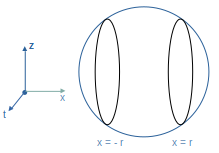
\includegraphics[scale=0.75]{Kr.png}
    \caption{$K_{r}$ in black.}
    \label{fig:Kr}
\end{figure}



Moreover, 
\begin{equation*}
\mbox{let }A_\theta = \begin{bmatrix}
\cos\theta & -\sin\theta & 0\\
\sin\theta & \cos\theta & 0\\
0 & 0 & 1
\end{bmatrix},    
\end{equation*}
 the rotation around the third coordinate and
 
\begin{equation*}
A'_\theta = \begin{bmatrix}
\cos\theta & -\sin\theta & 0 & 0\\
\sin\theta & \cos\theta & 0 & 0\\
0 & 0 & 1 & 0\\
0 & 0 & 0 & 1
\end{bmatrix},
\end{equation*}
the rotation "around the two last coordinates" which are classic examples of orthogonal matrices.

Besides that, we will call g the stereographic projection:

\begin{gather*}
\operatorname{g} : S^3 \rightarrow \hat{\R}^3 \\
\operatorname{g}(x_1, x_2, x_3, t) =
    \begin{cases}
        \infty, \text{ if } x_1 = x_2 = x_3 = 0, t = 1 \\
        \frac{1}{1 - t} (x_1, x_2, x_3), \mbox{ } c.c.
    \end{cases}
\end{gather*}

and

\begin{gather*}
\operatorname{g}_{(x,z,t)} = \restr{\operatorname{g}}{S^2_{(x,z,t)}}: S^2_{(x,z,t)} \rightarrow \R^3
\\
    \operatorname{g}_{(x,z,t)}(x, 0, z, t) =
    \begin{cases}
        \infty, \text{ if } x = z = 0, t = 1 \\
        \frac{1}{1 - t} (x, 0, z), \mbox{ } c.c.
    \end{cases}
\end{gather*}

Here we can easily see that g$_{(x,z,t)}$ is the stereographic projection sending the 2-sphere S$^2_{(x,z,t)}$ to the 2-plane 
\begin{equation*}
    \{(x,y,z) \in \R^4 : y = 0 \}.
\end{equation*}

And then, since K$_{r}$ is on S$^2_{(x,z,t)}$, we can define
\begin{equation*}
\famcirc_{r} := \operatorname{g}_{(x,z,t)}[K_{r}],    
\end{equation*}
being the stereographic projection acting on two symmetrical vertical circles on the 2-sphere, will be two Apollonian circles on the xz-plane of $\R^3$ [See the section \ref{TLF}], symmetric in relation to the $z$ axis, as you can see on figure \ref{fig:oi}. %não tenho certeza se era esse o nome do círculo ou da rede%

\begin{figure}[H]
    \centering
    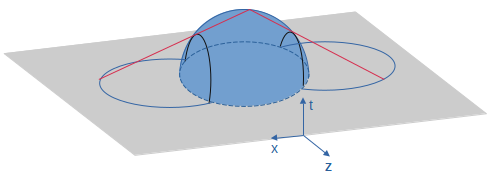
\includegraphics[scale=0.35]{projest.png}
    \caption{An illustration of $\operatorname{g}_{(x,z,t)}$, represented by the pink lines, with $K_{r}$ in black.}
    \label{fig:oi}
\end{figure}

And we can see that, $\forall (x,y,z,t) \in S^3,$
\begin{equation*}
    A_{\theta} \circ \operatorname{g}(x,y,z,t) = A_{\theta} \left(\frac{1}{1-t}(x,y,z)\right)
\end{equation*}
\begin{equation*}
    = \frac{1}{1-t} A_{\theta}(x,y,z)
\end{equation*}
\begin{equation*}
    = \operatorname{g}(A_{\theta}(x,y,z),t)
\end{equation*}
\begin{equation*}
    = \operatorname{g}\circ A'_{\theta}(x,y,z,t) 
\end{equation*}

noting that $(A_{\theta}(x,y,z),t)$ is in the domain of $g$, i.e. $(A_{\theta}(x,y,z),t) \in S^3$ because:
\begin{equation*}
    ||(A_{\theta}(x,y,z),t)||^2 = ||A_{\theta}(x,y,z)||^2 + t^2 = \langle A_{\theta}(x,y,z) \; , \; A_{\theta}(x,y,z) \rangle + t^2 
\end{equation*}
\begin{equation*}
    = \langle (x,y,z) \; , \; (x,y,z) \rangle + t^2 = x^2 + y^2 + z^2 + t^2 = 1
\end{equation*}

since $(x,y,z,t) \in S^3$ and $A_{\theta}$ is an orthogonal matrix.

With all this, we have:

\begin{equation*}
    \operatorname{g} \circ A'_{\theta}[K_{r}] = A_{\theta} \circ \operatorname{g}[K_{r}] = A_{\theta} \circ \operatorname{g}_{(x,z,t)}[K_{r}] = A_{\theta}[\famcirc_{r}]
\end{equation*}

And then:

\begin{equation*}
    \bigcup\limits_{0 \leq \theta \leq 2\pi} A_{\theta}[\famcirc_{r}] = \bigcup\limits_{0 \leq \theta \leq 2\pi} \operatorname{g} \circ A'_{\theta}[K_{r}] = \operatorname{g}\left(\bigcup\limits_{0 \leq \theta \leq 2\pi} A'_{\theta}[K_{r}]\right)
\end{equation*}

But C$_{r}$ is two circles on 
\begin{equation*}
\{(x,y,z) \in \R^3 : y = 0\},    
\end{equation*}
symmetric in relation to the $z$ axis, so the union of all the rotations around the $z$ axis 
\begin{equation*}
    \left(\bigcup\limits_{0 \leq \theta \leq 2\pi} A_{\theta}[\famcirc_{r}]\right)
\end{equation*}
will give us a ring torus in $\R^3$.

And:
\begin{equation*}
\bigcup\limits_{0 \leq \theta \leq 2\pi} A'_{\theta}[K_{r}] = T_{r} = \{(a,b,c,d) \in \R^4 : a^2+b^2=r^2 \mbox{ and } c^2+d^2=1-r^2\},
\end{equation*}
remembering that
\begin{equation*}
    K_{r} = \{(x,y,z,t) \in \R^4 : y=0, x^2=r^2, z^2+t^2 = 1-r^2\}:
\end{equation*}
$\subseteq$ : $\forall (x,0,z,t) \in K_{r}, \forall \theta \in [0,2\pi]$,
\begin{equation*}
    A'_{\theta}(x,0,z,t) = (x \cos\theta, x \sin{\theta}, z, t) \mbox{ with } x^2 = r^2 \mbox{ and } z^2+t^2=1-r^2.
\end{equation*}
\begin{equation*}
\mbox{ Since } (x \cos\theta)^2+(x \sin\theta)^2=x^2=r^2 \mbox{ and } z^2+t^2=1-r^2, A'_{\theta}(x,0,z,t) \in T_{r}.
\end{equation*}
$\supseteq$ : $\forall (x,y,z,t) \in T_{r}$,\\
\begin{equation*}
    \mbox{ we have } x^2+y^2=r^2 \mbox{ and } z^2+t^2=1-r^2,
\end{equation*}
\begin{equation*}
\mbox{ let } \hat{\theta} \mbox{ be } \arccos\left(\frac{x}{r}\right), \mbox{ so } \sin \hat{\theta} = \frac{y}{r}.    
\end{equation*}
\begin{equation*}
\mbox{ Therefore, }  (x,y,z,t) = (r \cos\hat{\theta}, r \sin\hat{\theta}, z, t) = A_{\hat{\theta}}(r,0,z,t).
\end{equation*}
\begin{equation*}
\mbox{ Since } z^2+t^2=1-r^2, (r,0,z,t) \in K_{r}, \mbox{ therefore } (x,y,z,t) \in A_{\hat{\theta}}(K_{r})
\end{equation*}

For r = 0, 1; we already know that the image will be a circle since the stereographic projection, being basically a restriction of a inversion, sends a circle in a circle.

But the same previous demonstration can be applied, with
\begin{equation*}
T_0=\{(x,y,z,t) \in \R^4 : x=y=0, z^2+t^2=1\},    
\end{equation*}
\begin{equation*}
T_1=\{(x,y,z,t) \in \R^4 : z=t=0, x^2+y^2=1\}    
\end{equation*}
so 
\begin{equation*}
    K_0=T_0 \subseteq \R^3_{(x,z,t)},
\end{equation*}
\begin{equation*}
    K_1=\{(-1,0,0,0),(1,0,0,0)\}
\end{equation*}
note that $K_1$ is the 2 foci of the Apollonian family of circles,

\begin{figure}[H]
    \centering
    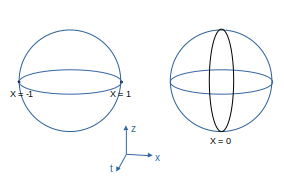
\includegraphics[scale=0.50]{K0K1.png}
    \caption{In black, $K_1$ on the left and $K_0$ on the right.}
    \label{fig:K0K1}
\end{figure}

so
 \begin{equation*}
    \famcirc_0=\{(x,z,t) \in \R^3 : x=t=0\}, 
 \end{equation*}
 \begin{equation*}
    \famcirc_1=\{(-1,0,0); (1,0,0)\}, 
 \end{equation*}
 notable cases of the stereographic projection,
 
 \begin{figure}[H]
    \centering
    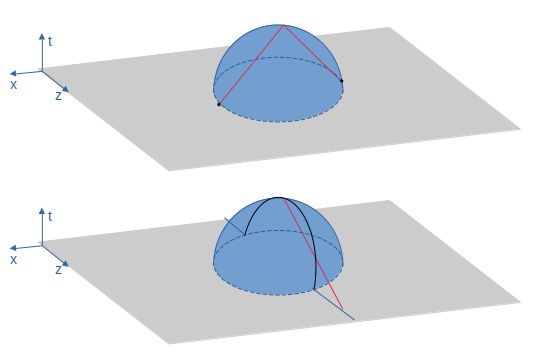
\includegraphics[scale=0.50]{C0C1.png}
    \caption{Above, $\famcirc_1$, and below, $\famcirc_0$ being "constructed" by the stereographic projection.}
    \label{fig:C0C1}
\end{figure}
 
 and then
 \begin{equation*}
 \operatorname{g}[T_0]=\famcirc_0
 \end{equation*}
 \begin{equation*}
 \operatorname{g}[T_1]=\{(x,z,t) \in \R^3 : z=0, x^2+t^2=1\},
 \end{equation*}
 circles on $\R^3$, being the line a circle that passes through infinity.

\begin{figure}[H]
    \centering
    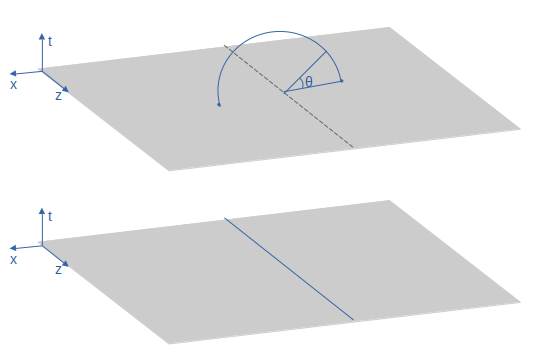
\includegraphics[scale=0.50]{gC0gC1.png}
    \caption{Above, g$[T_1]$ being "constructed" by union of rotations of C$_1$, and below, g$[T_0]$.}
    \label{fig:gC0gC1}
\end{figure}

In conclusion, each Hopf torus is sent to a ring torus in $\R^3$ by the stereographic projection, and the decomposition of $S^3$ in Hopf tori is sent to a union of all the rotations of the decomposition of the plane in Apollonian circles.
\end{proof}